\documentclass[bachelor, och, coursework, times]{SCWorks}
% параметр - тип обучения - одно из значений:
%    spec     - специальность
%    bachelor - бакалавриат (по умолчанию)
%    master   - магистратура
% параметр - форма обучения - одно из значений:
%    och   - очное (по умолчанию)
%    zaoch - заочное
% параметр - тип работы - одно из значений:
%    referat    - реферат
%    coursework - курсовая работа (по умолчанию)
%    diploma    - дипломная работа

				%    pract2      - отчет по практике, 2 курс, бакалавриат, магистратура
				%    pract3      - отчет по практике, 3 курс, бакалавриат
				%    pract4      - отчет по практике, 4 курс, бакалавриат
				%    practpreddip - отчет по преддипломной практике, 4 курс (= pract3 или nir) 
%    nir      - отчет о научно-исследовательской работе
%    autoref    - автореферат выпускной работы
%    assignment - задание на выпускную квалификационную работу
%    review     - отзыв руководителя
%    critique   - рецензия на выпускную работу
% параметр - включение шрифта
%    times    - включение шрифта Times New Roman (если установлен)
%               по умолчанию выключен
\usepackage[T2A]{fontenc}
\usepackage[utf8]{inputenc}
%\usepackage[utf8]{inputenc}
\usepackage{graphicx}
\usepackage[sort,compress]{cite}
\usepackage{amsmath}
\usepackage{amssymb}
\usepackage{amsthm}
\usepackage{fancyvrb}
\usepackage{longtable}
\usepackage{array}
\usepackage[english,russian]{babel}
%Красиво оформляет программый код внутри текста
\usepackage{minted}
\usepackage[dvipnames]{xcolor}
\definecolor{mygray}{gray}{0.9}
%Конец офорормления

\setminted{       % установка параметров по умолчанию для команд бибилиотеки minted
%	bgcolor=codebg, % установка цвета фона программного кода
	linenos=true,   % включение номеров строк в листингах
	numbersep=5pt,  % промежуток между номерами строк и началом строк листинга
	breaklines}     % автоматические переносы строк (когда строки не умещаются)

%\usemintedstyle{bw} % включение черно-белого стиля программного кода

% выделение ссылок цветом. чтобы включить- true
\usepackage[colorlinks=false]{hyperref}

\renewcommand{\rmdefault}{cmr} % курсив и полужирный включаются здесь.
\newcommand{\eqdef}{\stackrel {\rm def}{=}}

\newtheorem{lem}{Лемма}

\begin{document}

% Кафедра (в родительном падеже)
\chair{теории функций и стохастического анализа} 
\chairr{кафедра теории функций и стохастического анализа} % для практик!!!!
%\chairr{завод "Тантал"}% для практик!!!!

%Тема работы

\title{Правила оформления курсовых и дипломных работ}

% Курс
\course{2}

% Группа
\group{251}

\department{механико-математического факультета}

% Специальность/направление код - наименование
%\napravlenie{01.03.02 "--- Прикладная математика и информатика}
\napravlenie{38.03.05 "--- Бизнес-информатика}
%%\napravlenie{09.04.03 "--- Прикладная информатика}

% Для СТУДЕНТКИ!!!. Для работы студента следующая команда не нужна.
\studenttitle{Студентки}

% Фамилия, имя, отчество в родительном падеже
\author{Логаткиной Марии Михайловны}

% Заведующий кафедрой
\chtitle{д.\,ф.-м.\,н., доцент} % степень, звание
\chname{С.\,П.\,Сидоров}

%Научный руководитель (для реферата преподаватель проверяющий работу)
\satitle{доцент, к.\,ф.-м.\,н.} %должность, степень, звание
\saname{М.\,Г.\,Плешаков} % для 451 гр
%\saname{А.\,К.\,Смирнов} % для 412 гр

% Руководитель практики от организации (только для практики,
% для остальных типов работ не используется)

%\patitle{руководитель направления АРМ}
%\paname{Д.\,Э.\,Кнутов}

% Семестр (только для практики, для остальных
% типов работ не используется)
\term{3}

% Наименование практики (только для практики, для остальных
% типов работ не используется)
%\practtype{производственная(базовая)}

% Продолжительность практики (количество недель) (только для практики,
% для остальных типов работ не используется)
%\duration{4}

% Даты начала и окончания практики (только для практики, для остальных
% типов работ не используется)
\practStart{1.07.2024}
\practFinish{14.07.2024}

% Год выполнения отчета
\date{2025}

\maketitle

%Включение нумерации рисунков, формул и таблиц по разделам
% (по умолчанию - нумерация сквозная)
% (допускается оба вида нумерации)
%\secNumbering


\tableofcontents

% Раздел "Обозначения и сокращения". Может отсутствовать в работе
%\abbreviations
%\begin{description}
%    \item $|A|$  "--- количество элементов в конечном множестве $A$;
 %   \item $\det B$  "--- определитель матрицы $B$;
 %   \item ИНС "--- Искусственная нейронная сеть;
 %   \item FANN "--- Feedforward Artifitial Neural Network
%\end{description}

% Раздел "Определения". Может отсутствовать в работе
%\definitions

% Раздел "Определения, обозначения и сокращения". Может отсутствовать в работе.
% Если присутствует, то заменяет собой разделы "Обозначения и сокращения" и "Определения"
%\defabbr


% Раздел "Введение"
\intro
%Пример введения для курсовой работы
Целью настоящей работы является создание примера оформления студенческой работы средствами системы \LaTeX.

Поставлена задача оформить документ в соответствии:
\begin{itemize}
    \item со стандартом СТО 06.02-2019 Порядком выполнения, структурой и правилами оформления курсовых работ (проектов) и выпускных квалификационных работ, принятых в Саратовском государственном университете в 2019 году;
    \item с правилами оформления титульного листа отчета о прохождении практики в соответствии со стандартом СТО 1.01-2005.
\end{itemize}
%Далее следует привести краткую характеристику каждого раздела работы
В первом разделе работы приведены правила оформления работы по стандарту, в частности, рассматривается оформление рисунков и таблиц.

Во втором разделе работы более подробно изучаются способы набора математического текста, а именно .... (привести примеры)

Третий раздел работы содержит пример практического применения средств \LaTeX к фрагменту текста из математического анализа (программирования, алгебры и т.п.)

%%%%%%%%%%%%%%%%%%%%%%%%%%%%%%%%%%%%%%%%%%%%%%%%%%%%%%%%%%%%%%%%%%%%%%%%%%%%%%%%%%%%%%%%%%%%%%%%%%
%  пример для отчетов по практике для бакалавриата 2, 3 курсов

Целью учебной ознакомительной практики(заменить на соответствующую) <<Правила оформления курсовых и дипломных работ>> (заменить на свою) является создание примера оформления студенческой работы средствами системы \LaTeX.

Поставлена задача оформить документ в соответствии:
\begin{itemize}
    \item со стандартом СТО 06.02-2019 Порядком выполнения, структурой и правилами оформления курсовых работ (проектов)
    и выпускных квалификационных работ, принятых в Саратовском государственном университете в 2019 году;
    \item с правилами оформления титульного листа отчета о прохождении практики в соответствии со стандартом СТО 1.01-2005.
\end{itemize}

При решении поставленных задач (Во время прохождения практики) и при подготовке отчета были использованы источники [1--N]
% N количество источников в списке литературы, для отчета норма не установлена, но от пяти было бы неплохо.
% эту фразу можно не писать, если вы гарантированно расставите ссылки на ВСЕ источники внутри текста отчета.

%%%%%%%%%%%%%%%%%%%%%%%%%%%%%%%%%%%%%%%%%%%%%%%%%%%%%%%%%%%%%%%%%%%%%%%%%%%%%%%%%%%%%%%%%%%%%%%%%%
%  пример для отчетов по производственной базовой практике для бакалавриата 4 курса
Тема производственной базовой практики <<Название практики>>.

Целью производственной базовой практики <<Название  практики>>  являлось углубление и закрепление знаний, полученных в процессе обучения и приобретение необходимых навыков
по реализации полученных знаний в трудовой деятельности с использованием современных программно-аппаратных средств в составе научно-
производственного (или производственного) коллектива <<название организации, которой проходили практику>>, отделе, подразделении Название.

 Дайте краткую характеристику деятельности организации или отдела, в котором проходила практика.

 Основной вид деятельности Отдела Название состоит в (разработке ПП, разработке сайтов, обслуживании банковской деятельности и т.д.)

В работе были поставлены следующие задачи:(При прохождении практики передо мной были поставлены задачи)
\begin{itemize}
  \item изучение инструментов web-разработки (проектирование сайта, подключение необходимых модулей, подключение сервисов аналитики);
  \item изучение платформ для создания web-сайта (Tilda - конструктор, Wix- HTML5, PrestaShop - интернет-магазин);
  \item разработка и создание web-сайта компании и его поддержка (работа по техническому заданию);
  \item организация и управление работы в удаленном доступе (установка программы TeamViewer).
\end{itemize}

При решении поставленных задач (Во время прохождения практики) и при подготовке отчета были использованы источники [1--N]
% N количество источников в списке литературы, для отчета норма не установлена, но от пяти было бы неплохо.
% эту фразу можно не писать, если вы гарантированно расставите ссылки на ВСЕ источники внутри текста отчета.

% конец примера для отчетов по производственной базовой практике для бакалавриата 4 курса
%%%%%%%%%%%%%%%%%%%%%%%%%%%%%%%%%%%%%%%%%%%%%%%%%%%%%%%%%%%%%%%%%%%%%%%%%%%%%%%%%%%%%


\section{Правила оформления, выдержки из стандарта}

6.1.1 Курсовая работа (проект) и выпускная квалификационная работа (далее - работа) должна быть выполнена с использование компьютера и принтера на
одной стороне листа белой бумаги формата А4 шрифтом Times New Roman через
полтора интервала.
Цвет шрифта должен быть черным, высота цифр, букв и других знаков -
размером 14 пт (кеглей).
Текст работы следует печатать, соблюдая следующие размеры полей: левое
– 25 мм, правое – 15 мм, верхнее и нижнее – 20 мм.

Объем курсовой работы (проекта), как правило, составляет 20-30 страниц,
объем выпускной квалификационной работы бакалавра, специалиста – 40-60
страниц, магистра – 50-90 страниц.

Количество страниц, отводимых на каждый раздел работы, определяется
студентом по согласованию с научным руководителем (руководителем).
Допускается использовать компьютерные возможности для акцентирования
внимания на определениях, терминах, формулах и других важных особенностях
путем применения разных начертаний шрифта (курсив, полужирный, полужирный
курсив, разрядка и др.).

6.1.2 Опечатки, описки и графические неточности, орфографические, синтаксические и речевые ошибки, обнаруженные в процессе выполнения работы,
допускается исправлять закрашиванием корректором и нанесением на том же
месте исправленного текста (графики).
Повреждения листов, помарки, следы не полностью удаленного прежнего
текста (графики), орфографические, синтаксические и речевые ошибки не допускаются.

6.1.3 Работа должна быть подписана исполнителем. Подпись и дата ставятся исполнителем после списка использованных источников.

\subsection{Основные требования к изложению материала}

6.2.1 Текст работы должен быть кратким, четким, логически последовательным и не допускать двусмысленных толкований.

6.2.2 В работе должны применяться научные и научно-технические термины,
обозначения и определения, установленные соответствующими стандартами, а
при их отсутствии - общепринятые в научной и научно-технической литературе.

В тексте работы не допускается применять:
обороты разговорной речи, техницизмы, профессионализмы;
для одного и того же понятия различные научные и научно-технические
термины, близкие по смыслу (синонимы), если синонимические обозначения не
являются общепринятыми;
произвольные словообразования;
сокращения слов, кроме тех, которые установлены правилами русской
орфографии, стандартами, а также в данной работе

\subsection{Оформление рисунков и таблиц}

6.8 Иллюстрации
6.8.1 К иллюстрациям относят графики, схемы, компьютерные распечатки, диаграммы. Их следует располагать непосредственно после
текста, в котором они упоминаются впервые, или на следующей странице.

На все иллюстрации должны быть даны ссылки в тексте.

6.8.3 Иллюстрации, за исключением иллюстраций приложений, следует нумеровать арабскими цифрами сквозной нумерацией.
Если рисунок один, то он обозначается «Рисунок 1».
Иллюстрации при необходимости могут иметь наименование и пояснительные данные (подрисуночный текст). Слово «Рисунок», его номер и через тире
наименование помещают после пояснительных данных и располагают в центре
под рисунком без точки в конце.
Пример – Рисунок 1 - Детали прибора

Допускается нумеровать иллюстрации в пределах раздела. В этом случае
номер иллюстрации состоит из номера раздела и порядкового номера иллюстрации, разделенных точкой: Рисунок 1.1.
Иллюстрации каждого приложения обозначают отдельной нумерацией арабскими цифрами с добавлением перед цифрой обозначения приложения: Рисунок
А.3.

6.8.4 При ссылках на иллюстрации следует писать «... в соответствии с
рисунком 2» при сквозной нумерации и «... в соответствии с рисунком 1.2» при
нумерации в пределах раздела.

6.9 Таблицы

6.9.2 Таблицу следует располагать непосредственно после текста, в котором
она упоминается впервые, или на следующей странице.
Наименование таблицы, при его наличии, должно отражать ее содержание,
быть точным, кратким.
Наименование таблицы следует помещать над таблицей слева, в одну строку
с ее номером через тире.

6.9.3 На все таблицы должны быть ссылки в тексте. При ссылке следует
писать слово «таблица» с указанием ее номера.
6.9.4 Таблицу с большим числом строк допускается переносить на другой
лист. При переносе части таблицы на другой лист слово «Таблица», ее номер и
наименование указывают один раз слева над первой частью таблицы, а над
другими частями также слева пишут слова "Продолжение таблицы" и указывают
номер таблицы


6.9.6 Таблицы (за исключением таблиц приложений) следует нумеровать
арабскими цифрами сквозной нумерацией.
Допускается нумеровать таблицы в пределах раздела. В этом случае номер
таблицы состоит из номера раздела и порядкового номера таблицы, разделенных
точкой.
Таблицы каждого приложения обозначают отдельной нумерацией арабскими
цифрами с добавлением перед цифрой обозначения приложения.
Если в работе одна таблица, то она должна быть обозначена «Таблица 1»
или «Таблица B.1», если она приведена в приложении В.


6.11 Список использованных источников
6.11.1 Сведения об источниках приводятся в соответствии с требованиями
ГОСТ 7.1, ГОСТ 7.80 и ГОСТ 7.82.

Примеры библиографического описания в списке использованных источников
приведены в файле thesis.bib, например,
 \cite{Bari_Stechkin-1956}, \cite{Bari-1955}, \cite{Volosivez-2007},  \cite{Golubov_Efimov_Skvorzov},
Электронные ресурсы \cite{MSDN}, \cite{Wiki}.


 
\section{Пример оформления текста}
\subsection{Пример основных элементов математического текста}
Внутритекстовая формула $\frac{1}{\varepsilon^*}=\frac{1}{\varepsilon_\infty}-\frac{1}{\varepsilon_0}$.


Пример одиночной ссылки на литературу~\cite{Yoffe_1993_AP_42_173}. Пример множественной ссылки на литературу~\cite{Efros_1982_FTP_16_7_1209,Anselm_1978,Segall_1968,Agranovich_1983,Mishchenko_1996,Skvortsov_2008}.
Еще множественная ссылка~\cite{Perelman_2003_math:0307245, Nielsen_2010_1006.2735}. Пример ссылки на Приложение~\ref{pril-1}.
\begin{equation}
	F(x)=\int\limits_a^bf(x)\,dx.
\end{equation}

Ссылка на рисунок~\ref{fig:f}.
\begin{figure}[!ht]
	\centering
	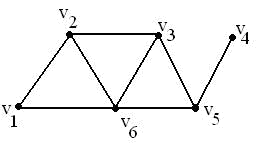
\includegraphics[width=6cm]{fig2.png}
	\caption{\label{fig:f}%
	Подпись к рисунку}
\end{figure}

Если разность энергий электронно"=дырочных уровней $E_2-E_1$ близка к энергии предельного оптического фотона $\hbar\Omega_{LO}$, то в разложении волновых функций полного гамильтониана можно ограничиться нулевым приближением для всех состояний, за исключением близких по значению к $E_2$. Волновые функции последних представляют собой следующие комбинации почти вырожденных состояний\cite{Skvortsov_2008}.

\subsection{Еще элементы математического текста}
Нейрон является составной частью нейронной сети. Он состоит из
элементов трех типов: умножителей (синапсов), сумматора и
нелинейного преобразователя. Синапсы осуществляют связь между
нейронами, умножают входной сигнал на число, характеризующее силу
связи (вес синапса). Сумматор выполняет сложение сигналов,
поступающих по синаптическим связям от других нейронов, и внешних
входных сигналов. Нелинейный преобразователь реализует нелинейную
функцию одного аргумента "--- выхода сумматора. Эта функция
называется функцией активации или передаточной функцией. На рисунке~\ref{neuron} приведено строение одного нейрона.

Нейрон в целом реализует скалярную функцию векторного аргумента.
Математическая модель нейрона:
\[
	 s = \sum\limits_{i = 1}^n w_i x_i + b,
\]
\[
	 y = f(s),
\]
где $w_i $ "--- вес синапса; $i = 1,\ldots ,n$; $b$ "--- значение
смещения; $s$ "--- результат суммирования; $x_i $ "--- $i$-тый
компонент входного вектора (входной сигнал), \linebreak $i = 1,\ldots, n$;
$y$ "--- выходной сигнал нейрона; $n$ "--- число входов нейрона;
$f(s)$ "--- нелинейное преобразование (функция активации).
\begin{figure}[ht]
	\centering
	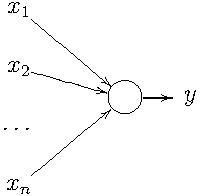
\includegraphics{Neuron}
	\caption{Нейрон}\label{neuron}
\end{figure}

В качестве функции активации нейронов берут обычно одну из
следующих:
\begin{itemize}
	\item пороговая функция активации;
	\item экспоненциальная сигмоида;
	\item рациональная сигмоида;
	\item гиперболический тангенс.
\end{itemize}

Данные функции активации обладают таким важным свойством как
нелинейность. Нелинейность функции активации принципиальна для
построения нейронных сетей. Если бы нейроны были линейными
элементами, то любая последовательность нейронов также производила
бы линейное преобразование и вся нейронная сеть была бы
эквивалентна одному нейрону (или одному слою нейронов в случае
нескольких выходов). Нелинейность разрушает суперпозицию и
приводит к тому, что возможности нейросети существенно выше
возможностей отдельных нейронов.

\subsection{Снова математический текст}
Опишем самую популярную архитектуру
"--- многослойный персептрон с последовательными связями и
сигмоидальной функцией активации (\foreignlanguage{english}{Feedforward Artifitial Neural
Network, FANN}).

В многослойных нейронных сетях с последовательными связями нейроны
делятся на группы с общим входным сигналом "--- слои. Стандартная
сеть состоит из $L$ слоев, пронумерованных слева направо. Каждый
слой содержит совокупность нейронов с едиными входными сигналами.
Внешние входные сигналы подаются на входы нейронов входного слоя
(его часто нумеруют как нулевой), а выходами сети являются
выходные сигналы последнего слоя. Кроме входного и выходного слоев
в многослойной нейронной сети есть один или несколько скрытых
слоев, соединенных последовательно в прямом направлении и не
содержащих связей между элементами внутри слоя и обратных связей
между слоями. Число нейронов в слое может быть любым и не зависит
от количества нейронов в других слоях. Архитектура нейронной сети
прямого распространения сигнала приведена на рисунке~\ref{net1}.

На каждый нейрон первого слоя подаются все элементы внешнего
входного сигнала. Все выходы нейронов $i$-го слоя подаются на
каждый нейрон слоя $i+1$.

Нейроны выполняют взвешенное суммирование элементов входных
сигналов. К сумме прибавляется смещение нейрона. Над результатом
суммирования выполняется нелинейное преобразование "--- функция
активации (передаточная функция). Значение функции активации есть
выход нейрона. Приведем схему многослойного персептрона. Нейроны
представлены кружками, связи между нейронами "--- линиями со
стрелками.

\begin{figure}[ht]
	\centering
	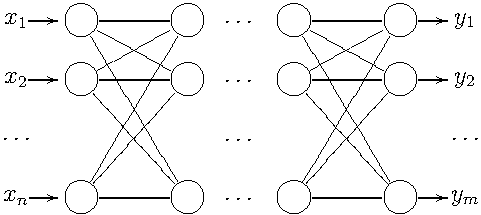
\includegraphics{NN-Scheme}
	\caption{Архитектура многослойной сети прямого
распространения}\label{net1}
\end{figure}

Функционирование сети выполняется в соответствии с формулами:
\[
	s_j^{\left[ k \right]} = \sum\limits_{i = 1}^{N_{k - 1} }
	{w_{ji}^{\left[ k \right]} y_i^{\left[ {k - 1} \right]} +
	b_j^{[k]} ,\ \ j = 1,\ldots ,N_k ,\ \ k = 1,\ldots ,L;}
\]
\[
	 y_j^{\left[ k \right]} = f(s_j^{\left[ k \right]} ),\ \ j =
	1,\ldots ,N_k ,\ \ k = 1,\ldots ,L-1,
\]
\[
	 y_j^{\left[ L \right]} = s_j^{\left[ L \right]} ,
\]
где
\begin{itemize}
	\item
		$y_i^{\left[ {k - 1} \right]}$ "--- выходной сигнал $i$-го нейрона
        $(k - 1)$-го слоя; \item $w_{ji}^{\left[ k \right]}$ "--- вес связи
        между $j$-м нейроном слоя $(k-1)$ и $i$-м нейроном $k$-го
        слоя;
	\item
		$b_j^{\left[ k \right]}$ "--- значение смещения $j$-го
        нейрона $k$-го слоя;
	\item
		$y = f(s)$ "--- функция активации;
	\item
		$y_j^{\left[ k \right]}$ "--- выходной сигнал $j$-го
		нейрона $k$-го слоя;
	\item
		$N_k$ "--- число узлов слоя $k$;
	\item
		$L$ "--- общее число основных слоев;
	\item
		$n = N_0$ "--- размерность входного вектора;
	\item
		$m = N_L$ "---
		размерность выходного вектора сети.
\end{itemize}

На рисунке~\ref{net2} представлена сеть прямого распространения
сигнала с 5 входами, 3 нейронами в скрытом слое и 2 нейронами в
выходном слое.
\begin{figure}[hb]
	\centering
	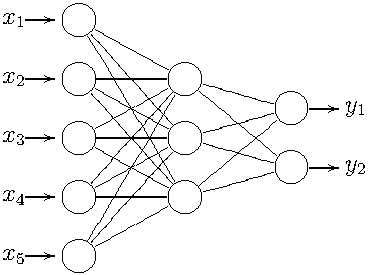
\includegraphics{NN-Persep}
	\caption{Пример нейронной сети}\label{net2}
\end{figure}


\section{Раздел с подразделами}
\subsection{Текст с формулами и леммой}

Обозначим $[y_0,y_1,\ldots,y_p;f]$ разделенную разность порядка $p$ функции $f$ по узлам $y_0<y_1<\ldots<y_p$.

Обозначим $L_pf(x;y_0,y_1,\ldots,y_p)$ интерполяционный полином Ньютона функции $f$ по узлам $y_0,y_1,\ldots,y_p$:
\begin{equation} \label{eq:ex01}
    L_pf(x;y_0,y_1,\ldots,y_p)=\sum_{j=0}^p[y_0, \ldots,y_{j};f]
    \cdot \prod_{i=0}^{j-1}(x-y_i), \ \ x-y_{-1}\eqdef 1
\end{equation}

\begin{lem} \label{lem:1}
    Если $0\leqslant x_0<x_1<\ldots <x_p\leqslant 1$ и
    $f\in C[0,1]$ удовлетворяет условиям
    \begin{enumerate}
        \item
            \label{it:1lem1}$f(x)\geqslant 0, \ x\in [0,1]$;
        \item
            \label{it:2lem1}
            $[y_0,\ldots,y_{p+1};f]\geqslant 0$
            для всех $y_i \in [0,1], \
            i=0,\ldots,p+1,$
    \end{enumerate}
    тогда
    \begin{equation}\label{eq:ex02}
        L_pf(x;x_0,\ldots,x_p)\geqslant 0
    \end{equation}
    для всех $x\in [x_{p-(2k+1)},x_{p-2k}]$,
    $k=0,\ldots,\left[p/2\right]$,
    $x_{-1} \eqdef -\infty$.
\end{lem}
\begin{proof}
    Возьмем $x \in [x_{p-(2k+1)},x_{p-2k}]$,\ \ $k=0,\ldots,\left[p/2
    \right]$.

    Из условия \ref{lem:1} леммы следует, что
    \begin{displaymath}
        [x_0,\ldots,x_{p-(2k+1)},x,x_{p-2k},\ldots,x_p;f] \geqslant
        0,
    \end{displaymath}
    т.~е.
    \begin{multline}\label{eq:ex03}
     \Delta_pf(x;x_0,\ldots,x_p)\eqdef
     \\ \eqdef
      \begin{vmatrix}
       1 & x_0   & x_0^2 & \cdots & x_0^p & f(x_0) \\
       \vdots  & \vdots & \vdots & \ddots & \vdots & \vdots \\
       1 & x_{p-(2k+1)} & x_{p-(2k+1)}^2 & \cdots & x_{p-(2k+1)}^p & f(x_{p-(2k+1)}) \\
       1 & x & x^2 & \cdots & x^p & f(x) \\
       1 & x_{p-2k} & x_{p-2k}^2 & \cdots & x_{p-2k}^p & f(x_{p-2k}) \\
       \vdots  & \vdots & \vdots & \ddots & \vdots & \vdots \\
       1 & x_p & x_p^2 & \cdots & x_p^p & f(x_p) \\
      \end{vmatrix}
      \geqslant 0
    \end{multline}

    Из равенства
    \begin{equation*}
        \Delta_p f(x;x_0,\ldots,x_p)=(L_pf(x;x_0,\ldots,x_p)-f(x))
        \prod_{0\leqslant i<j\leqslant p}(x_j-x_i).
    \end{equation*}
	и \eqref{eq:ex03} следует, что
    \begin{displaymath}
        L_pf(x;x_0,\ldots,x_p)\geqslant f(x).
    \end{displaymath}

    С учетом условия \ref{it:1lem1} леммы мы получаем утверждение \eqref{eq:ex02}.
\end{proof}

\subsection{Название другого подраздела}
\subsubsection{Более мелкий подраздел}
Если разность энергий электронно"=дырочных уровней $E_2-E_1$ близка к энергии предельного оптического фотона $\hbar\Omega_{LO}$, то в разложении волновых функций полного гамильтониана можно ограничиться нулевым приближением для всех состояний, за исключением близких по значению к $E_2$.

\subsubsection{Текст с таблицей}
В таблице~\ref{table-1} представлены результаты сокращения словарей неисправностей для схем из каталога ISCAS'89.

\begin{table}[!ht]
	\small
	\caption{Результат сокращения словарей неисправностей при помощи масок} \label{table-1}
	\begin{tabular}{|l|c|c|c|c|r|r|r|}
		\hline 1 & 2& 3& 4& 5& 6& 7& 8\\
		\hline S298 & 177 & 1932 & 341964 & 61 & 10797 & 3,16\% & 0,61\\
		\hline S344 & 240 & 1397 & 335280 & 59 & 14160 & 4,22\% & 0,53\\
		\hline S349 & 243 & 1474 & 358182 & 62 & 15066 & 4,21\% & 0,60\\
		\hline S382 & 190 & 12444 & 2364360 & 55 & 10450 & 0,44\% & 3,78\\
		\hline S386 & 274 & 2002 & 548548 & 91 & 24934 & 4,55\% & 1,40\\
		\hline S400 & 194 & 13284 & 2577096 & 58 & 11252 & 0,44\% & 4,28\\
		\hline S444 & 191 & 13440 & 2567040 & 60 & 11460 & 0,45\% & 4,26\\
		\hline S510 & 446 & 700 & 312200 & 70 & 31220 & 10,00\% & 0,63\\
		\hline S526 & 138 & 13548 & 1869624 & 38 & 5244 & 0,28\% & 2,41\\
		\hline S641 & 345 & 5016 & 1730520 & 132 & 45540 & 2,63\% & 7,06\\
		\hline S713 & 343 & 3979 & 1364797 & 131 & 44933 & 3,29\% & 5,61\\
		\hline S820 & 712 & 21185 & 15083720 & 244 & 173728 & 1,15\% & 126,99\\
		\hline S832 & 719 & 21603 & 15532557 & 253 & 181907 & 1,17\% & 135,18\\
		\hline S953 & 326 & 322 & 104972 & 91 & 29666 & 28,26\% & 0,27\\
		\hline S1423 & 293 & 750 & 219750 & 93 & 27249 & 12,40\% & 0,57\\
		\hline S1488 & 1359 & 22230 & 30210570 & 384 & 521856 & 1,73\% & 541,69\\
		\hline
	\end{tabular}
\end{table}

\subsubsection{Текст с кодом программы}
Термин <<разреженная матрица>> впервые был предложен Гарри Марковицем. В 1989 он был награжден премией имени Джона фон Неймана в том числе и за вклад в теорию методов для разреженных матриц.

В большинстве источников, разреженной матрицей называется матрица, в которой мало ненулевых элементов. Это нельзя назвать определением из-за слова <<мало>>. В \cite{matrix_87} понятие разреженной матрицы определяется так: <<Мы можем называть матрицу разреженной, если применение к ней методов, описываемых в книге, экономит память и/или время>>. Таким образом, следует дать определение алгоритму для разреженных матриц. Алгоритмом для разреженных матриц будем называть алгоритм, у которого время работы и необходимый объем памяти зависят от количества ненулевых элементов в матрице.

Размерность квадратной матрицы $A$ будем обозначать $n$, а количество ненулевых элементов в ней $|A|$.

Плотные матрицы обычно хранятся в качестве двумерного массива $n\times n$. Будем обозначать такой массив a. Разреженные матрицы не стоит хранить таким способом из-за слишком большого потребления памяти, которая будет занята в основном нулевыми элементами.

Один из вариантов представления разреженных матриц в памяти компьютера "--- в виде трех массивов: \verb"column", \verb"value" и \verb"rowIndex". Размеры массивов \verb"column" и \verb"value" равны $|A|$. Размер \verb"rowIndex" равен $n+1$. Ненулевые элементы матрицы $A$ хранятся последовательно по строкам в этих массивах. Элемент \verb"column[i]" содержит номер столбца, в котором содержится \verb"i"-й ненулевой элемент, а \verb"value[i]" "--- его величину. Массив \verb"rowIndex[i]" содержит в себе индекс первого ненулевого элемента \verb"i"-й строки. Все ненулевые элементы \verb"i"-й строки содержатся в массивах \verb"column" и \verb"value" в элементах с индексами от \verb"rowIndex[i]" по \verb"rowIndex[i + 1]-1". Для удобства полагают \verb"rowIndex["$n$\verb"]"$=|A|$.

Для примера рассмотрим следующую матрицу:
\[
    \left(
    \begin{matrix}
        1 & 0 & 5 & 0 & 0 \\
        0 & 2 & 7 & 4 & 0 \\
        0 & 0 & 1 & 0 & 0 \\
        9 & 6 & 0 & 3 & 0 \\
        0 & 0 & 3 & 0 & 5
    \end{matrix}
    \right)
\]

Массивы \verb"column", \verb"value" и \verb"rowIndex" для этой матрицы представлены в таблице~\ref{tab:mat-arrays}.
\begin{table}[ht]\small
	\caption{Массивы \texttt{column}, \texttt{value} è \texttt{rowIndex}}\label{tab:mat-arrays}
	\begin{tabular}{|l|c|c|c|c|c|c|c|c|c|c|c|c|} \cline{2-13}
		\multicolumn{1}{c|}{} & 0 & 1 & 2 & 3 & 4 & 5 & 6 & 7 & 8 & 9 & 10 & 11 \\ \cline{2-13}\hline
		\verb"column" & 0 & 2 & 1 & 2 & 3 & 2 & 0 & 1 & 3 & 2 & 4 &  \\ \hline\hline
		\verb"value" & 1 & 5 & 2 & 7 & 4 & 1 & 9 & 6 & 3 & 3 & 5 &  \\ \hline\hline
		\verb"rowIndex" & 0 & 2 & 5 & 6 & 9 & 11 &  &  &  &  &  &  \\ \hline
	\end{tabular}
\end{table}

Неизвестный вектор и вектор правой части хранятся в виде массивов размера $n$. Массив неизвестного вектора обозначают \verb"x", а массив правой части "--- \verb"rhs".

Рассмотрим пример алгоритма для разреженных матриц. Алгоритм решения СЛАУ, представленной нижнетреугольной матрицей \verb"a", можно реализовать двумя вложенными циклами по \verb"n":
\begin{minted}[fontsize=\small]{Perl}
for(int i = 0; i $<$ n; ++i){
    x[i] = rhs[i];
    for(int j = 0; j $<$ i; ++j)
        x[i] -= a[i][j] * x[j];
    x[i] /= a[i][i];
} 
\end{minted}

Но, если матрица \verb"a" хранится в разреженном виде, то в данном алгоритме можно проходить только по ненулевым элементам \verb"a":
\begin{minted}[fontsize=\small]{Perl}
for(int i = 0; i $<$ n; ++i){
    x[i] = rhs[i];
    for(int j = rowIndex[i]; j $<$ rowIndex[i + 1] - 1; ++j)
        x[i] -= value[j] * x[column[j]];
    x[i] /= value[rowIndex[i + 1] - 1];
}
\end{minted}

В первом случае оценка времени работы будет $O(n^{2})$, а во втором $O(|A|)$.

Методы для разреженных матриц основаны на следующих главных принципах~\cite{matrix_87}:

\begin{enumerate}
    \item  Хранятся только ненулевые элементы матрицы.
    \item  Выполняются только те преобразования, которые действительно что"=то изменяют. В примере не имеет смысла вычитать из \verb"x[i]" значение \verb"x[j]*a[i][j]", если \verb"a[i][j]" равно нулю.
    \item  Число <<новых элементов>>, возникающих, например, во время исключения Гаусса, стараются уменьшить путем перестановок строк и столбцов матрицы.
\end{enumerate}


% Раздел "Заключение"
\conclusion
В настоящей работы приведен пример оформления студенческой работы средствами системы \LaTeX.

Показано, как можно оформить документ в соответствии:
\begin{itemize}
    \item с правилами оформления курсовых и выпускных квалификационных работ, принятых в Саратовском государственном университете в 2019 году;
    \item с правилами оформления титульного листа отчета о прохождении практики в соответствии со стандартом.
\end{itemize}

%%%%%%%%%%%%%%%%%%%%%%%%%%%%%%%%%%%%%%%%%%%%%%%%%%%%%%%%%%%%%%%%%%%%%%%%%%%%%%%%%%%%%%%%%%%%%%%%%%
%  пример для отчетов по производственной базовой практике для бакалавриата 4 курса

В результате прохождения практики "Название практики"  были получены знания и сформированы профессиональные навыки, необходимые в трудовой деятельности компании предприятия (организации, АО, ООО ... )"Название места прохождения" на
должности Системного администратора. Также были решены поставленные задачи (задачи из введения)по созданию и настройки web-сайта фирмы, а также установке
возможности по работе в удаленном режиме.

Таким образом, производственная практика способствовала формированию следующих компетенций:%%%% ВНИМАНИЕ!!! ниже указаны компетенции для БИ. ПМИ уточните состав компетенций у руководителя, либо возьмите сами на сайте мехмата в разделе Практика.
%%% можно выбрать не менее трех компетенций или оставить все

ОК – 6 Способность работать в коллективе, толерантно воспринимая социальные, этнические, конфессиональные и культурные различия;

ОПК – 2 Способность находить организационно – управленческие решения и готов нести за них ответственность; готов к ответственному и целеустремленному решению поставленных профессиональных задач во взаимодействии с обществом, коллективом, партнерами;

ОПК – 3 Способность работать с компьютером как средством управления информацией, работать с информацией из различных источников, в том числе в глобальных компьютерных сетях;

ПК – 13 Умение проектировать и внедрять компоненты ИТ-инфраструктуры предприятия, обеспечивающие достижение стратегических целей и поддержку бизнес-процессов;

ПК – 19 Умение готовить научно-технические отчеты, презентации, научные публикации по результатам выполненных исследований.


%%%%%%%%%%%%%%%%%%%%%%%%%%%%%%%%%%%%%%%%%%%%%%%%%%%%%%%%%%%%%%%%%%%%%%%%%%%%%%%%%%%%%%%%%%%%%%%%%%


%Библиографический список, составленный вручную, без использования BibTeX
%
%\begin{thebibliography}{99}
%  \bibitem{Ione} Источник 1.
%  \bibitem{Itwo} Источник 2.
%\end{thebibliography}

%Библиографический список, составленный с помощью BibTeX
%
\bibliographystyle{ugost2003}



\bibliography{thesis}

% Окончание основного документа и начало приложений
% Каждая последующая секция документа будет являться приложением
\appendix

\section{Нумеруемые объекты в приложении}

\begin{table}[!ht]
	\footnotesize
	\caption{Results of pass-fail dictionary reduction with the help
	of masks} \label{table-2}
	\begin{tabular}{|p{1.5cm}|
	                 p{1.5cm}|
	                 p{1.5cm}|
	                 p{1.5cm}|
	                 p{1cm}|
	                 p{1.5cm}|
	                 p{1.5cm}|
	                 p{1cm}|}
		\hline \centering Circuit & Number of modelled faults & Number of test
		vectors in the test set & The volume of pass-fail dictionary,
		\linebreak bit & The volume of found mask & The volume of
		masked dictionary, \linebreak bit & \raggedright \% of pass-fail dictionary
		& CPU running time, \linebreak min
		\\
		\hline S298 & 177 & 322 & 56994 & 30 & 5310 & 9,32\% & 0,07\\
		\hline S344 & 240 & 127 & 30480 & 29 & 6960 & 22,83\% & 0,04\\
		\hline S349 & 243 & 134 & 32562 & 35 & 8505 & 26,12\% & 0,05\\
		\hline S382 & 190 & 2074 & 394060 & 28 & 5320 & 1,35\% & 0,43\\
		\hline S386 & 274 & 286 & 78364 & 65 & 17810 & 22,73\% & 0,26\\
		\hline S400 & 194 & 2214 & 429516 & 32 & 6208 & 1,45\% & 0,99\\
		\hline S444 & 191 & 2240 & 427840 & 30 & 5730 & 1,34\% & 0,98\\
		\hline S526 & 138 & 2258 & 311604 & 28 & 3864 & 1,24\% & 0,61\\
		\hline S641 & 345 & 209 & 72105 & 58 & 20010 & 27,75\% & 0,24\\
		\hline S713 & 343 & 173 & 59339 & 58 & 19894 & 33,53\% & 0,19\\
		\hline S820 & 712 & 1115 & 793880 & 147 & 104664 & 13,18\% & 9,09\\
		\hline S832 & 719 & 1137 & 817503 & 151 & 108569 & 13,28\% & 9,20\\
		\hline S953 & 326 & 14 & 4564 & 13 & 4238 & 92,86\% & 0,01\\
		\hline S1423 & 293 & 150 & 43950 & 58 & 16994 & 38,67\% & 0,15\\
		\hline S1488 & 1359 & 1170 & 1590030 & 158 & 214722 & 13,50\% & 26,69\\
		\hline
	\end{tabular}
\end{table}

\begin{equation}
  F(x)=\int\limits_a^bf(x)\,dx.
\end{equation}


\begin{figure}[!ht]
	\centering
	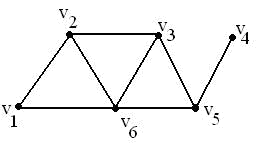
\includegraphics[width=6cm]{fig2.png}
	\caption{\label{fig:f3}%
	Подпись к рисунку}
\end{figure}


\begin{table}[!ht]
\caption{}
\begin{tabular}{|c|c|}
  \hline
  0 & 1\cr
  \hline
  1 & 0\cr
  \hline
\end{tabular}
\end{table}


\section{Листинг программы}\label{pril-1}
Код приложения \verb"task.pl".

\inputminted{perl}{task.pl}


\section{Многостраничная таблица}

\noindent
{\small
\begin{longtable}[l]{|>{\centering}p{2cm}|
								     >{\raggedright}p{6cm}|
								     >{\centering}p{2cm}|
								     >{\centering}p{2cm}|}
\caption{ГОСТ DIN ISO "--- Таблица соответствия стандартов}\label{tab:longtab}
\cr\hline
\textbf{Стандарт ГОСТ} & \centering\textbf{Наименование} & \textbf{Стандарт DIN} & \textbf{Стандарт ISO} \cr
\hline
1 &  \centering 2  & 3  &  4 \endfirsthead
\caption*{Продолжение таблицы~\ref{tab:longtab}}\cr
\hline
1 &  \centering 2  & 3  &  4  \cr\hline\endhead \hline
ГОСТ 397-79 & Шплинты & DIN 94 & ISO 1234 \cr \hline
ГОСТ 1144-80 & Шурупы с полукруглой головкой & DIN 96DIN 7981 & ISO 7049 \cr \hline
ГОСТ 1145-80 & Шурупы с потайной головкой & DIN 97DIN 7982 & ISO 7050 \cr \hline
ГОСТ 1146-80 & Шурупы с полупотайной головкой & DIN 95DIN 7983 & ISO 7051 \cr \hline
ГОСТ 1476-93 & Винты установочные с коническим концом и прямым шлицем классов точности А и В & DIN 553 & ISO 7434 \cr \hline
ГОСТ 1477-93 & Винты установочные с плоским концом и прямым шлицем классов точности А и В & DIN 438DIN 551 & ISO 4766ISO 7436 \cr \hline
ГОСТ 1478-93 & Винты установочные с цилиндрическим концом и прямым шлицем классов точности А и В & DIN 417 & ISO 7435 \cr \hline
ГОСТ 1481-84 & Винты установочные с шестигранной головкой и цилиндрическим концом классов точности А и В & DIN 561 & ~ \cr \hline
ГОСТ 1482-84 & Винты установочные с квадратной головкой и цилиндрическим концом классов точности А и В & DIN 479 & ~ \cr \hline
ГОСТ 1485-84 & Винты установочные с квадратной головкой и засверленным концом классов точности А и В & DIN 479 & ~ \cr \hline
ГОСТ 1486-84 & Винты установочные с квадратной головкой и ступенчатым концом со сферой классов точности А и В & DIN 480 & ~ \cr \hline
ГОСТ 1488-84 & Винты установочные с квадратной головкой и буртиком классов точности А и В & DIN 478 & ~ \cr \hline
ГОСТ 1491-80 & Винты с цилиндрической головкой классов точности А и В & DIN 84 & ISO 1207 \cr \hline
ГОСТ 3032-76 & Гайки-барашки & DIN 315 & ~ \cr \hline
ГОСТ 3033-79 & Болты откидные & DIN 444 & ~ \cr \hline
ГОСТ 3057-90 & Пружины тарельчатые & DIN 2093 & ~ \cr \hline
ГОСТ 3070-88 & Канат стальной двойной свивки типа ТК конструкции 6х19 (1+6+12)+1 о.с. & DIN 3060 & ~ \cr \hline
ГОСТ 3128-70 & Штифты цилиндрические незакаленные & DIN 7DIN 6325 & ISO 2338ISO 8734 \cr \hline
ГОСТ 3129-70 & Штифты конические незакаленные & DIN 1 & ISO 2339 \cr \hline
ГОСТ 4751-73 & Рым-болты & DIN 580 & ISO 3266 \cr \hline
ГОСТ 5915-70 & Гайки шестигранные стальные класса точности В & DIN 555DIN 934 & ISO 4032ISO 4033ISO 8673ISO 8674 \cr \hline
ГОСТ 5916-70 & Гайки шестигранные низкие класса точности В & DIN 439DIN 936 & ISO 4035ISO 4036ISO 8675 \cr \hline
ГОСТ 5918-73 & Гайки шестигранные прорезные и корончатые класса точности В & DIN 935 & EN ISO 7035EN ISO 7036EN ISO 7037 \cr \hline
ГОСТ 5919-73 & Гайки шестигранные прорезные и корончатые низкие класса точности В & DIN 937 & EN ISO 7038 \cr \hline
ГОСТ 5927-70 & Гайки шестигранные класса точности А & DIN 555DIN 934 & ISO 4032ISO 4034ISO 8673 \cr \hline
ГОСТ 5932-73 & Гайки шестигранные прорезные и корончатые класса точности А & DIN 935DIN 937 & EN ISO 7035EN ISO 7036EN ISO 7037 \cr \hline
ГОСТ 6393-73 & Гайки круглые с отверстиями на торце "под ключ" класса точности А & DIN 1816 & ~ \cr \hline
ГОСТ 6402-70 & Шайбы пружинные & DIN 127 & ~ \cr \hline
ГОСТ 6958-78 & Шайбы увеличенные. Классы точности А и С & DIN 440DIN 9021 & ISO 7094ISO 7093-1ISO 7093-2 \cr \hline
ГОСТ 7786-81 & Болты с потайной головкой и квадратным подголовком класса точности С & DIN 608 & ~ \cr \hline
ГОСТ 7795-70 & Болты с шестигранной уменьшенной головкой и направляющим подголовком, класс точности В & ~ & ~ \cr \hline
\end{longtable}
}

\end{document}
